%%%%%%%%%%%%%%%%%%%%%%%%%%%%%%%%%%%%%%%%%%%%%%%%%%%%%%%%%%%%%%%%%%%%%%%
%%%%%%%%%%%%%%%%%%%%%%%%%%%%%%%%%%%%%%%%%%%%%%%%%%%%%%%%%%%%%%%%%%%%%%%
%%%%%                                                                 %
%%%%%     <file_name>.tex                                             %
%%%%%                                                                 %
%%%%% Author:      <author>                                           %
%%%%% Created:     <date>                                             %
%%%%% Description: <description>                                      %
%%%%%                                                                 %
%%%%%%%%%%%%%%%%%%%%%%%%%%%%%%%%%%%%%%%%%%%%%%%%%%%%%%%%%%%%%%%%%%%%%%%
%%%%%%%%%%%%%%%%%%%%%%%%%%%%%%%%%%%%%%%%%%%%%%%%%%%%%%%%%%%%%%%%%%%%%%%

\chapter{System Overview}

\section{Sensors}

\todo{Diagram with all sensors etc.}

\subsection{Laser Distance Sensors}

In total four laser distance sensors were used to assess the vehicle attitude in relation to the rail.

Two high precision sensors were employed to measure the lateral alignment to the track at the front and the back of the pod. These sensors provided the input for the yaw controller in order to actively ensure that the pod is correctly aligned with the track and not exercising an torque on the rail.

Two smaller form-factor sensors were also installed at the front and back of the pod to measure the pods vertical alignment. These were mostly used to assess the performance of the clamping system.

\subsection{Pressure Sensors}

\subsubsection{Ambient pressure sensors}

A high-precision pressure sensor was installed to monitor the ambient pressure. Two further ambient pressure sensors were installed inside of each high-voltage battery pack, as these were pressurized. If the pressure inside the battery packs drops too low the battery cells could be permanently damaged. Therefore, it was necessary to monitor these values and re-pressurize the pod's environment in the event of a leak.

\subsubsection{Braking pressure sensors}

Four high-pressure sensors were installed in the braking system. One in each braking piston to measure the pressure with which the brakes actuate and to determine their status. Additionally, one sensor was installed in each reservoir holding the pressure used to engage the brakes in order to monitor brake health. The braking system consisted of two independent hydraulic systems for redundancy, thus two sets of sensors were necessary.

\subsection{Navigational Sensors}

Two laser contrast sensors were used to detect optical marking on the wall of the test tube. The optical markings occur in intervals of 30m and can therefore be used to determine the location of the pod along the tube and calculate it's velocity.

\section{Propulsion system} \label{spec_inverter}

Four two-phase electric motors are used to accelerate the pod. Each is driven by a separate inverter. The inverters are controlled via a CAN bus and two digital safety signals. The RFE signal enables the inverter and the RUN signal connects the high voltage from the battery to the motor. The inverter can be configured over the CAN bus. Subsequently, both torque and speed commands can be given to the inverters to drive the motors. Furthermore, the inverters provide telemetry over CAN including the following:

\begin{itemize}
    \item Inverter status
    \item DC bus voltage
    \item DC current
    \item Motor RPMs
    \item Motor RMS current
    \item Inverter temperature
    \item Motor temperature
\end{itemize}

\section{Battery Management System (BMS)}

Two battery management modules (one in each battery pack) are responsible for balancing the battery cells and monitoring them. These modules are also connected to a CAN bus and provide the following telemetry over it:

\begin{itemize}
    \item High-voltage isolation status
    \item Battery Pack Voltage
    \item Discharge/Charge current
    \item Lowest cell voltage
    \item Highest cell temperature
\end{itemize}

\section{Telemetry and Control Panel}

To monitor the pod a network is made available inside the tube. The pod connects to this network and must transmit all telemetry necessary to assess the pod's state and make sure it is safe. In addition, the pod is controlled over the network. Should the connection to the pod fail at any point, the pod must enter a safe state immediately. To control the pod and display telemetry a control panel application was developed.

\begin{figure}[H]
  \centering 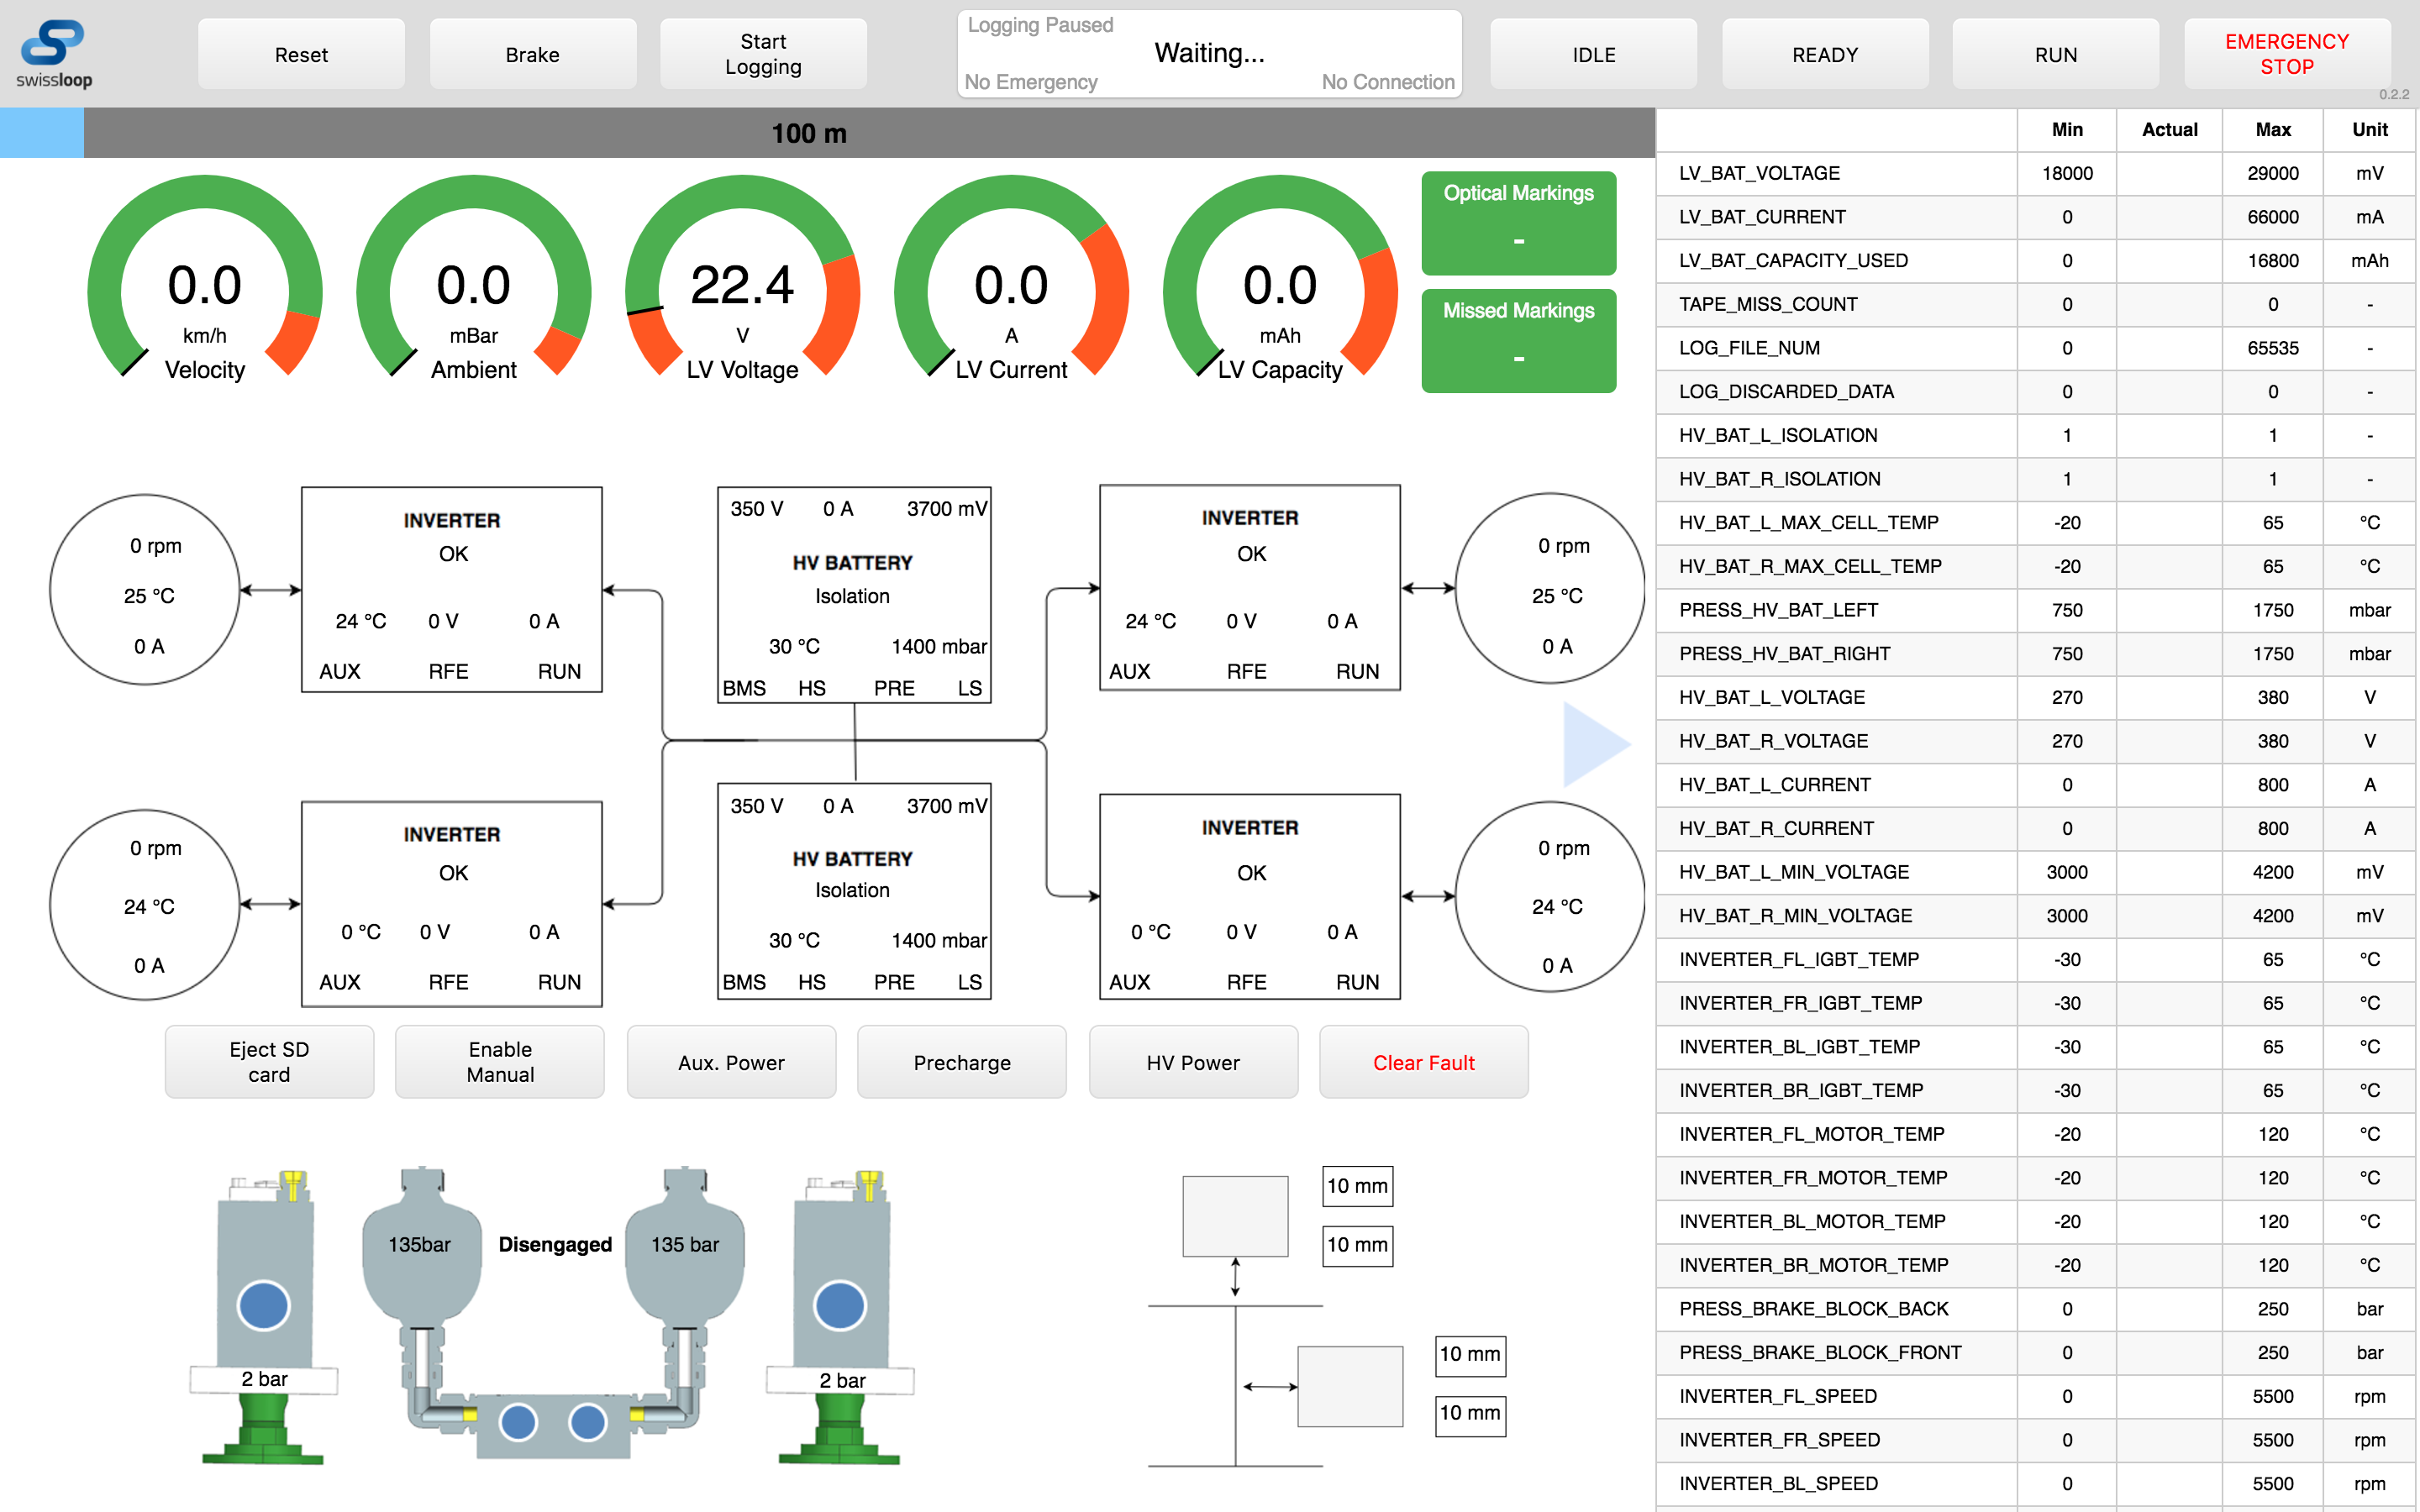
\includegraphics[width=1.0\textwidth]{./figures/Screen_Shot_Control_Panel.png}
  \caption{Screen shot of the control panel.}
\end{figure}

\section{Data Logging}

In order to verify the pod's performance and diagnose possible failures, we wanted to be able to log as much data as possible. Therefore, we set a goal of logging all sensor data that comes into the system.

\todo{Maybe add screenshot of plotting software?}

\section{Control and State Machine}

Overall, the pod is controlled by a finite state machine (FSM). The FSM must incorporate all critical safety checks and is also used to allow the pod to complete the run autonomously. In order to improve testability, the FSM should have the minimum number of states necessary for the desired functionality. To this end we also decided to minimize the number of automatic state transitions, minimizing the risk of bugs in the implementation.

\section{Correctness and Testability}

The highest priority for this system was to ensure correctness and safety. Therefore it was important to minimize sources of errors and implement the system with testability in mind. Tests include unit tests for individual control sequences and algorithms, as well as functional tests.

\section{Platform}

The hardware platform used for this project is a combination of a custom designed PCB and a Texas Instruments Launchpad (LAUNCHXL-F28379D) featuring the TMS320F28379D micro-controller. The Launchpad provides a sold basis which includes all the components necessary to run the micro-controller. It then plugs into the custom PCB which accommodates all the necessary external components and incorporates connectors for all sensors and actuators.

\todo{References to MCU/Launchpad}

\begin{figure}[H]
  \centering 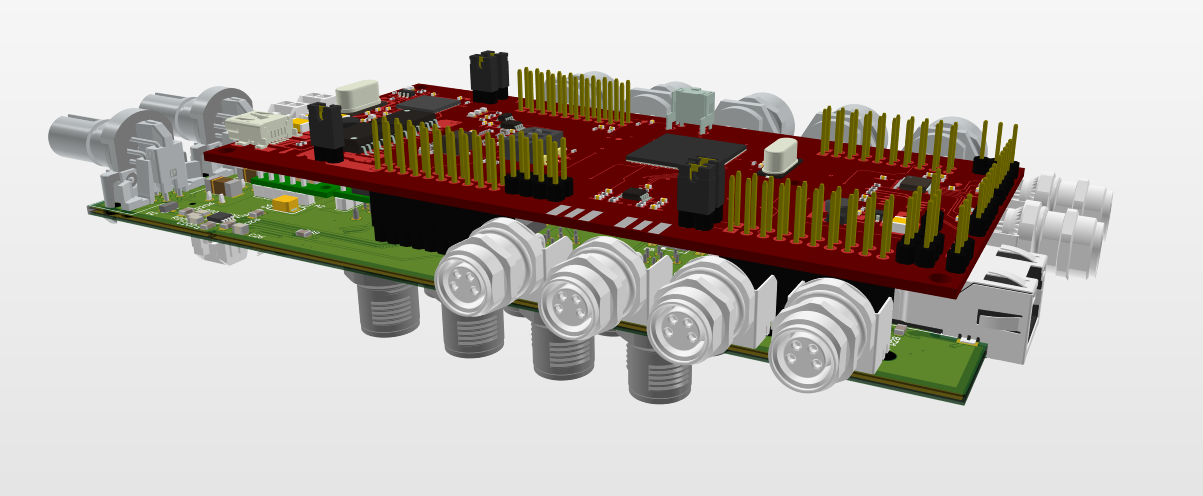
\includegraphics[width=1.0\textwidth]{./figures/pcb.png}
  \caption{Custom PCB with Texas Instruments Launchpad.}
\end{figure}

\subsection{Micro-controller}

The Texas Instruments TMS320F28379D was chosen as it provides high performance in terms of processing with two C28x CPU cores running at 200 MHz and two Control Law Accelerators (CLA). In addition, it incorporates a wide range of versatile peripherals covering most types of interfaces used in the system. Furthermore, this processor is a dual-core version of the single core TMS320F28377S which proved to work very well in Escher.

Texas Instruments also provides a good Runtime Support Library (RTS) for C, as well as header files and support functions as part of ControlSUITE\todo {reference} making it easier to access device registers.

\subsection{Ethernet Controller}

To establish a network connection on the test track an Ethernet connection was required. Since the micro-controller is not equipped with an Ethernet interface it needed to be included externally.

After considering several options we decided on the WIZnet W5500 Ethernet Controller. Beyond providing Ethernet support it also incorporates hardware implementations of ICMP, ARP, IPv4, TCP, UDP and other protocols. This is advantageous as it offloads the computation necessary to run the network stack from the main processor, providing better performance. Furthermore, the chip is widely used and therefore has good community support.

The micro-controller communicates with the Ethernet Controller over SPI but the W5500 also provides an interrupt line which can be configured to provide interrupts on events such as incoming packages.

\subsection{SD-Card}

In order to log telemetry data a form of non-volatile memory was needed. The data must be easily accessible and quickly retrievable. The obvious and most suitable choice is an SD-card, as it can be integrated into the SPI bus and provides large amounts of storage. At the same time it can be easily plugged into a laptop in order to retrieve the data in the field.

\subsection{External Analog-To-Digital Converter (ADC)}

The pressure sensors on the pod produce analog signals that need to be converted. Additionally, the pod incorporates a set of low-voltage batteries and it is necessary to monitor their voltage and discharge current. Although the micro-controller features a built-in 12-bit ADC which could accomplish this task, we wanted to achieve higher precision using an external 24-bit ADC (ADS124S08). Communication with the ADC also runs over an SPI bus. However, the external ADC uses a different SPI mode than the Ethernet Controller and SD-card. Thus a separate SPI bus is required.

\subsection{RS485 Bus}

An objective in the design of this system, was to use as many digital sensors as possible. This was possible for both types of laser distance sensors used on the pod. Both support the RS485 serial bus. Using an appropriate RS485 transceiver, the Serial Communication Interface (SCI) of the micro-controller can be utilized almost natively to communicate with multiple sensors on a single RS485 bus. Unfortunately the two types of sensors use different bus settings and thus it was simpler to separate them into two buses with two sensors each.

RS485 utilizes differential signalling to transmit words asynchronously in the same format as the more widely used RS232 protocol. Since RS485 uses a single differential signal, it is only possible for one device to transmit at a time.

Using the RS485 bus standard means less analog signals that are more prone to interference. Furthermore, it also allows for higher precision, as there are no precision losses during to conversions.

\subsection{CAN Bus}

The motor-controllers (inverters) used on the pod are designed for automotive applications, while the Battery Management Systems (BMS) are designed for aerospace applications. Both systems are designed to use the CAN bus for control and telemetry. The micro-controller incorporates a CAN bus and transceiver on the Launchpad making communication with these devices possible without any additional hardware.

The main advantages of the CAN bus in this application are built-in bus arbitration and automatic retransmission. This allows devices on the CAN bus to transmit telemetry data asynchronously without the possibility of data loss.

%%% Local Variables: 
%%% mode: latex
%%% TeX-master: "../report_template"
%%% End: 
